\documentclass[tikz,border=5mm]{standalone}
\usepackage{tikz}
\usepackage{amsmath}
\usetikzlibrary{arrows.meta}

% Define arrow styles
\tikzset{
    myarrow/.style={-{Stealth[length=3mm]}, thick},
    gridline/.style={gray!30, thin},
}

\begin{document}
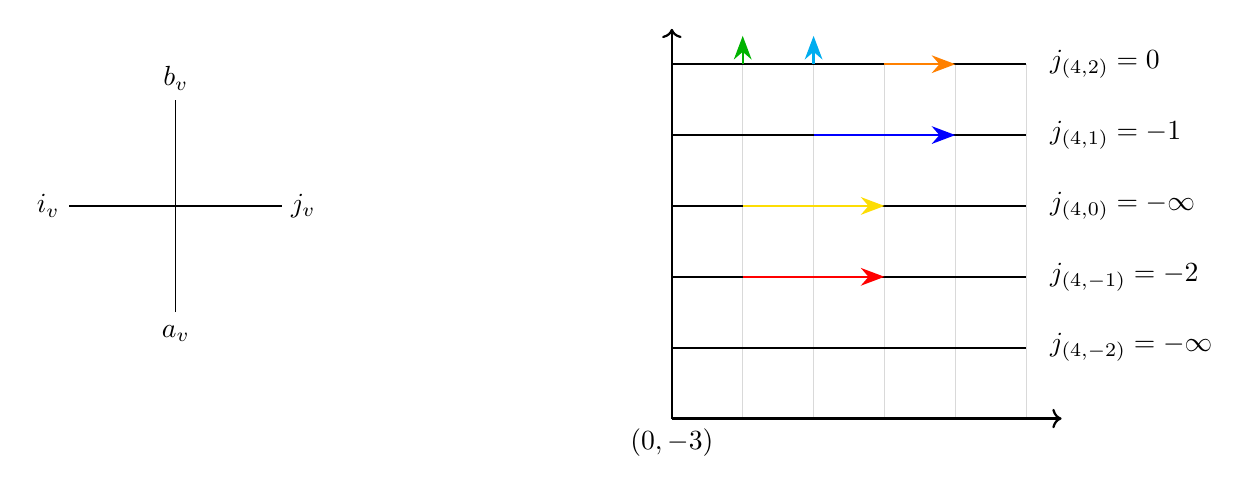
\begin{tikzpicture}[scale=0.9]
    % Left figure: Simple cross coordinate system
    \begin{scope}[shift={(-5,0)}]
        % Draw axes
        \draw[-] (-1.5,0) -- (1.5,0);
        \draw[-] (0,-1.5) -- (0,1.5);
        
        % Add labels
        \node at (0,-1.8) {$a_v$};
        \node at (0,1.8) {$b_v$};
        \node at (-1.8,0) {$i_v$};
        \node at (1.8,0) {$j_v$};
    \end{scope}
    
    % Right figure: Grid-based coordinate system with arrows and function values
    \begin{scope}[shift={(2,0)}]
        % Draw grid and coordinate axes
        \draw[gridline] (0,-3) grid (5,2);
        \draw[thick, ->] (0,-3) -- (5.5,-3);
        \draw[thick, ->] (0,-3) -- (0,2.5);
        
        % Draw horizontal lines and labels
        \foreach \y/\label/\idx in {-2/{j_{(4,-2)}=-\infty}/5, -1/{j_{(4,-1)}=-2}/4, 0/{j_{(4,0)}=-\infty}/3, 1/{j_{(4,1)}=-1}/2, 2/{j_{(4,2)}=0}/1} {
            \draw[thick] (0,\y) -- (5,\y);
            \node[right] at (5.2,\y) {$\label$};
        }
        
        % Add coordinate label
        \node[below] at (0,-3) {$(0,-3)$};
        
        % Draw colored arrows
        \draw[myarrow, red] (1,-1) -- (3,-1);
        \draw[myarrow, blue] (2,1) -- (4,1);
        \draw[myarrow, green!70!black] (1,2) -- (1,2.4);
        \draw[myarrow, cyan] (2,2) -- (2,2.4);
        \draw[myarrow, orange] (3,2) -- (4,2);
        \draw[myarrow, yellow!80!orange] (1,0) -- (3,0);
    \end{scope}
\end{tikzpicture}
\end{document}